As one of the focus points of this paper the choice of encoding parameters and the video preprocessing are of main importance. This section will first cover the two different encoding presets, go over the method which is used to derive the target bitrates and finalize with a description of the process automation.

\subsubsection{Encoding Presets}
We use the open x265 encoder for our experiment as it offers good performance and integration in the FFmpeg toolchain. Two different presets are used for the sequence encodings, a "na\"{\i}ve" (P.1) and an "expert" preset (P.2). The "na\"{\i}ve" preset is a simple \textit{CBR} (Constant Bitrate) encoding, whereas the "expert" preset is a 2-pass encoding with a Quality-Control pass followed by a Bitrate-Control pass.  Every sequence is encoded with both presets at 3 resolutions (540p, 1080p, 2160p) and 3 bitrates for each resolution. The following section goes into detail on how we select those bitrates.

\begin{figure}[htb!]
	\centering
	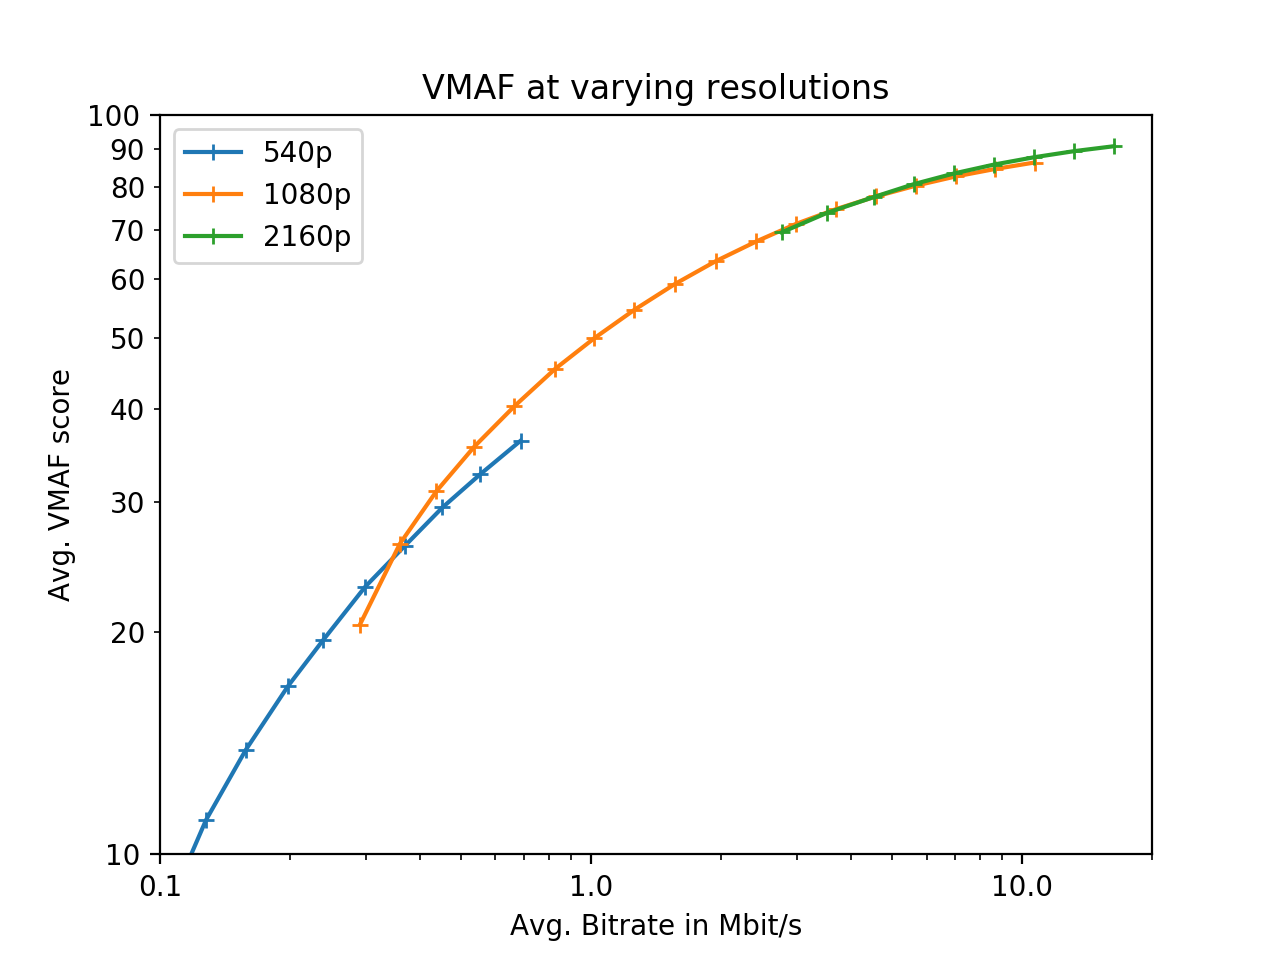
\includegraphics[width=3.5in]{vmaf_bitrates}
	\caption{Average \textit{VMAF} scores for 25 different bitrates at 3 resolutions. The encoded bitrates and the \textit{VMAF} scores are averaged between the 6 sequences and form the abscissa (Log) and ordinate respectively.}
	\label{fig:vmaf:bitrates}
\end{figure}

\subsubsection{Selection of Bitrates}
Video Multi-Method Assessment Fusion (\textit{VMAF}) is a full reference metric for estimating human perception of video quality \cite{lin2013:mmf}. We use \textit{VMAF} because it provides a better estimate of subjective quality than single metrics like \textit{SSIM} or \textit{VIF}.

To estimate relevant \textit{HEVC} encoding bitrates for our source content we sample the \textit{VMAF} scores at 25 bitrates on a logarithmic scale for our 3 different resolutions (540p, 1080p, 2160p). The reference sequences are resampled to a fixed 50 frames per seconds to avoid frame rate differences, while the distorted sequences are downsampled, encoded with \textit{CBR} rate control and upsampled to \textit{UHD-1} again using lanczos resampling. Both presets use 4:2:0 chroma subsampling to be close to the typical use-case of webvideo. The sampling requires 222 total sequences to be encoded with x265 and analyzed with the \textit{VMAF Development Kit} (VDK). This process takes around 18 hours (excluding download and cutting of the source material) on a current 10-Core x64 CPU.

The resulting \textit{VMAF} scores exhibit an overlap between different resolutions and the final encoding bitrates are chosen near those intersections. Figure \ref{fig:vmaf:bitrates} shows the sampled scores with the target rates in the background. We choose the target bitrates at least 2 bitrate-samples away from an intersection with the next quality, except for the lower 1080p-bound where it is not possible to lower the bitrate any further due to encoder restrictions. This should ensure a relevant sampling of the \textit{MOS}-bitrate space for the subjective test.

\begin{figure}[htb!]
	\centering
	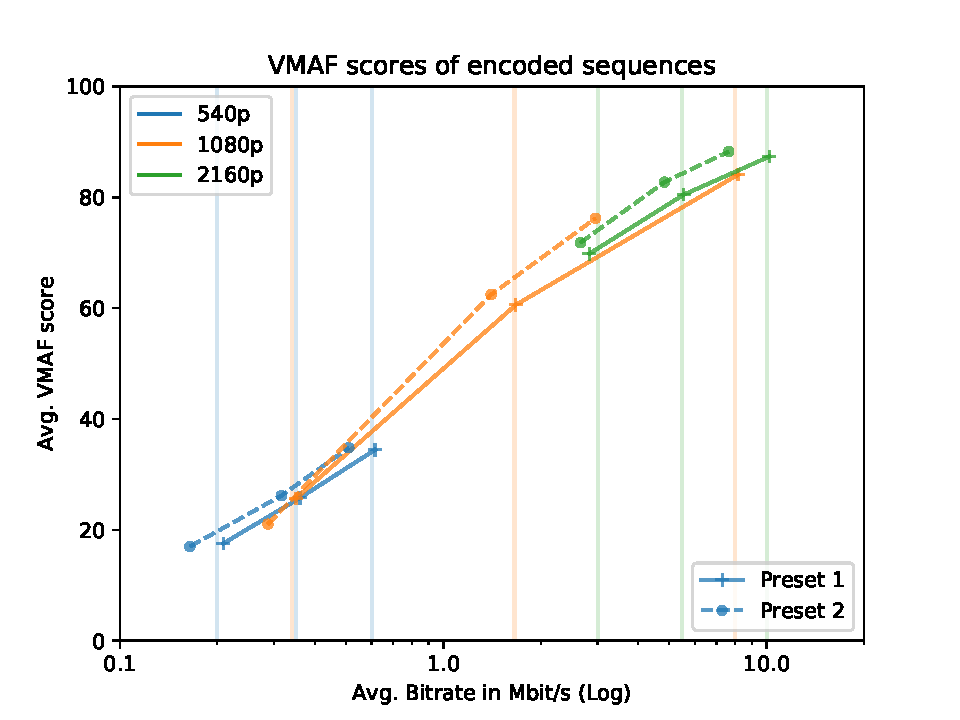
\includegraphics[width=3.5in]{vmaf_final}
	\caption{Average \textit{VMAF} scores of encoded videos for both presets. The encoded bitrates and the \textit{VMAF} scores are averaged between the 6 sequences for each preset and form the abscissa (Log) and ordinate respectively.}
	\label{fig:vmaf:encoded}
\end{figure}

The average \textit{VMAF} scores of the two presets at the chosen bitrates can be seen in Figure \ref{fig:vmaf:encoded}. The target bitrates can again be seen in the background. The scores of the "expert" preset are consistently higher than the ones for the "na\"{\i}ve" preset at matching bitrates. Furthermore the "expert" preset saves bitrate by resorting to an acceptable level of quality, while the "na\"{\i}ve" presets bitrates are very close to the targets.


\begin{figure}[bht!]
	\centering
	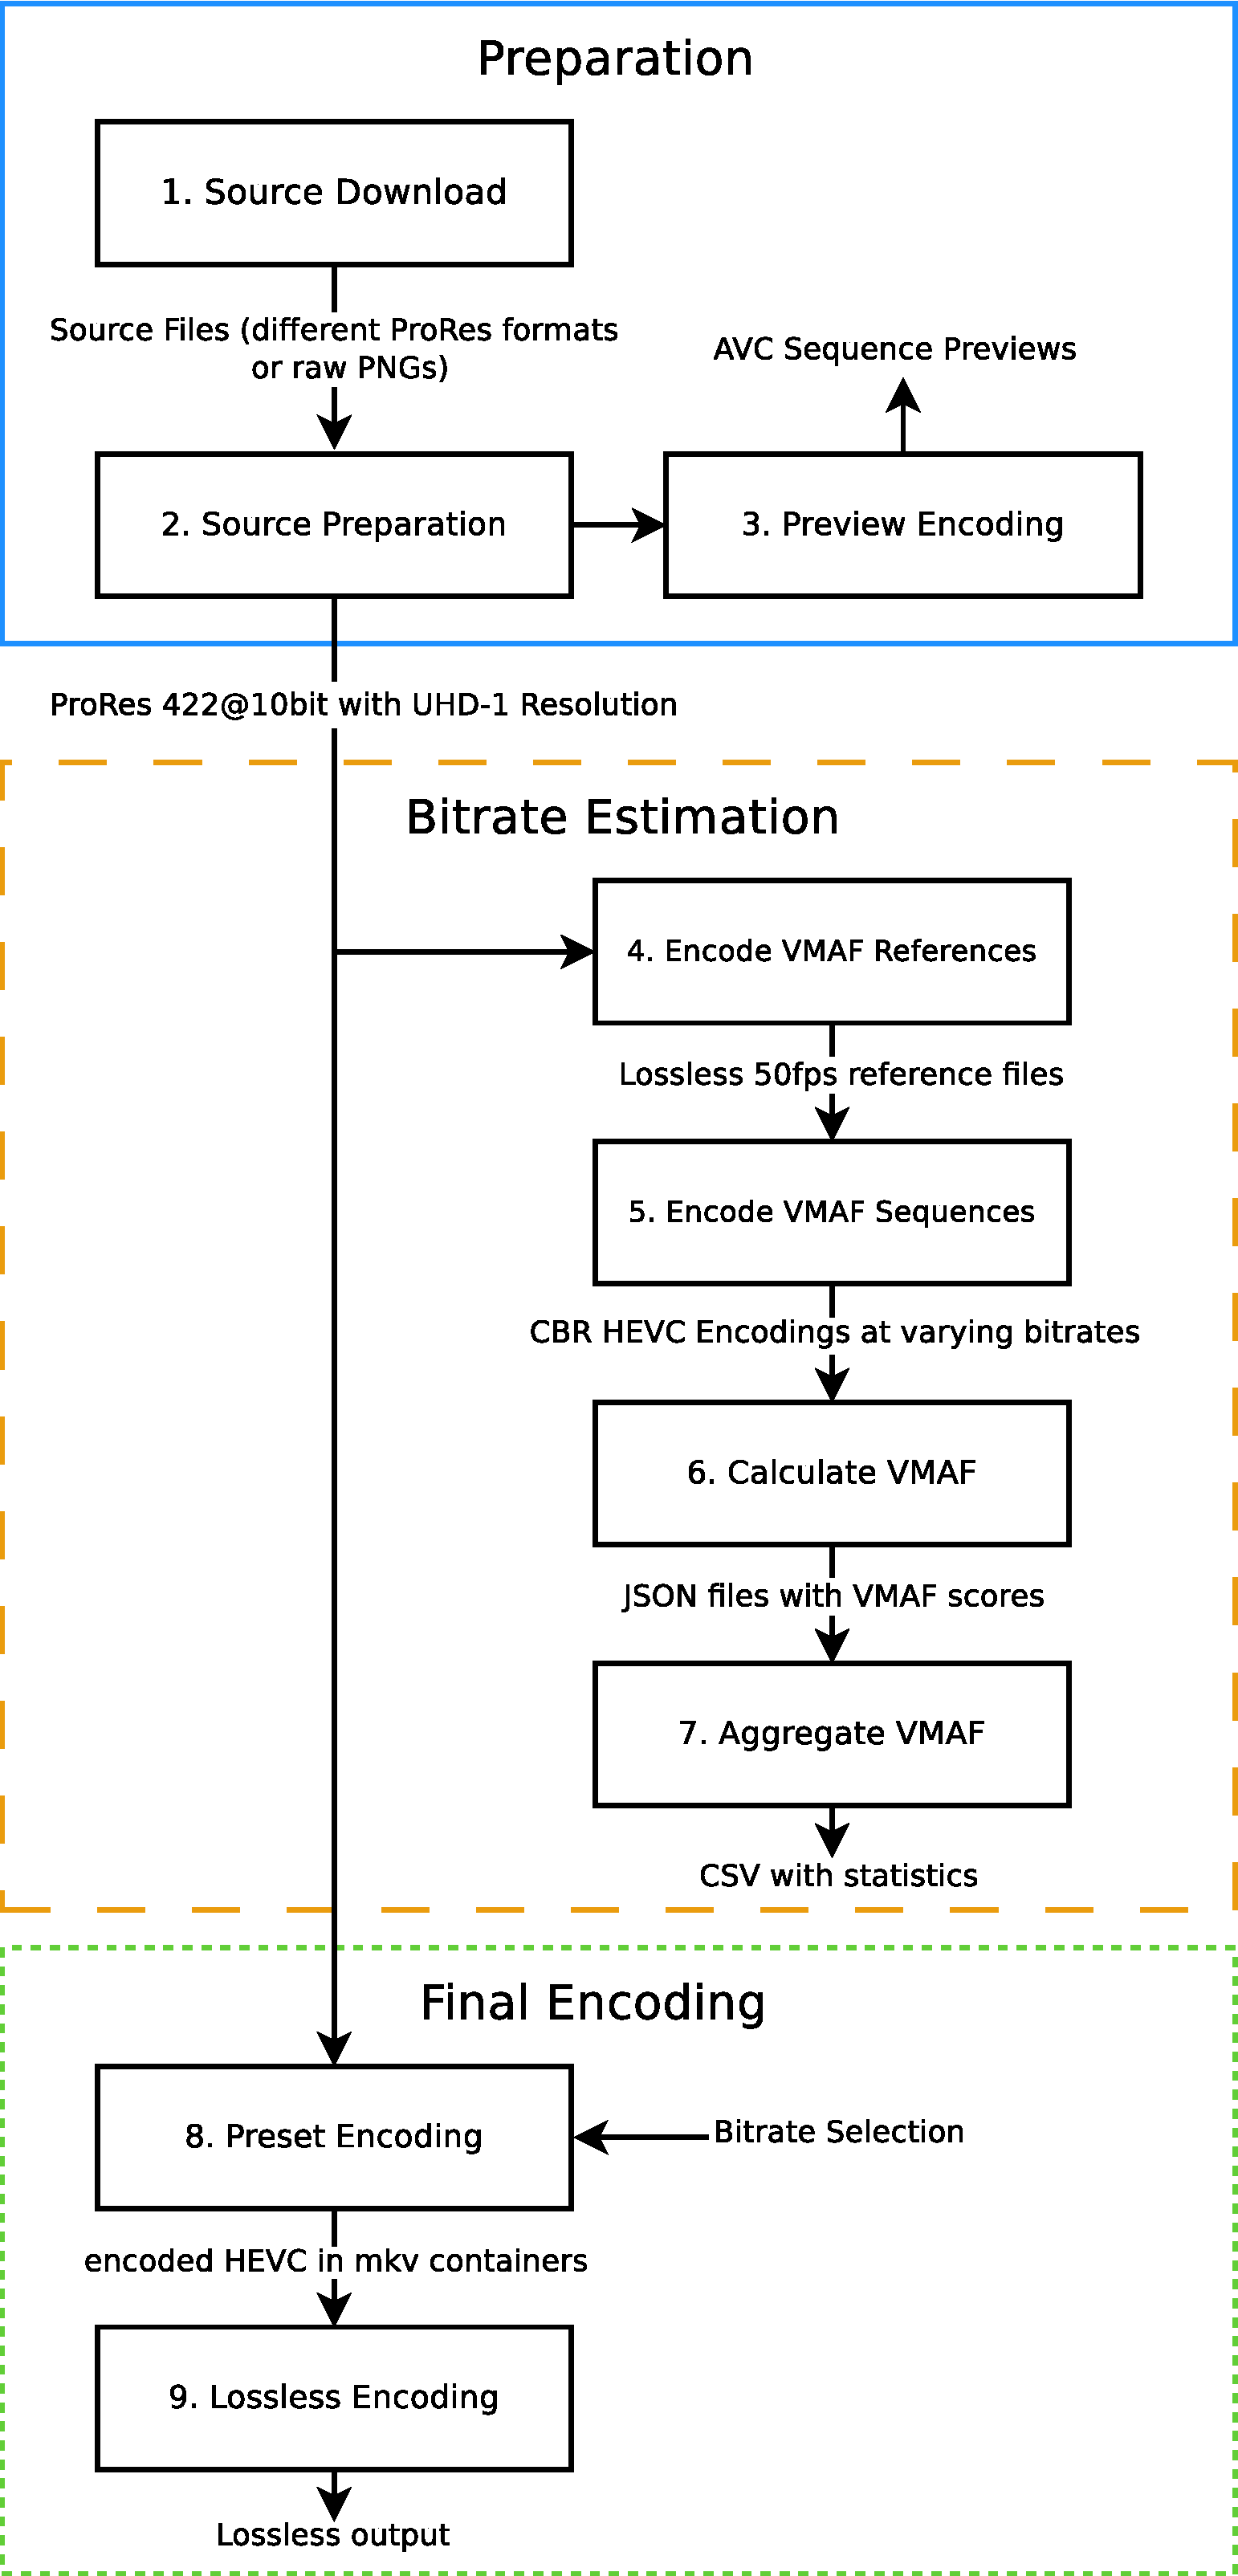
\includegraphics[width=2.5in]{automation}
	\caption{Automated processing and encoding workflow.}
	\label{fig:automation}
\end{figure}

\subsubsection{Encoding Automation}
We automate the whole process for downloading, preprocessing and encoding the source videos using pydoit \cite{web:pydoit}. This speeds up the turnaround time for changed parameters or sequences and also ensures that the encoded material can later be reproduced.

The whole process is illustrated in Figure \ref{fig:automation} and starts with the source preparation (A). After download of the sequences (1) they are cut to 10 seconds length and saved as ProRes HQ with \textit{UHD-1} resolution (2). Additionally, \textit{MPEG4-AVC} previews are generated at a lower resolution of 1440p to allow review of the sequences on slower devices.

After the initial processing the bitrate estimation is performed (B) using the \textit{VMAF} metric \cite{lin2013:mmf}. The videos are brought to the same frame rate of 50fps (4) and encoded with \textit{CBR} at 25 different bitrates (5). The average \textit{VMAF} score of each video is analyzed with the \textit{VMAF} Development Kit (VDK) \cite{web:vdk} and saved as a json file (6). All of the average scores are then aggregated into a single CSV for plotting and further analysis (7). The target bitrates can then derived from these scores.

The last step is the main encoding (C). It can only start after the target bitrates have been specified in the configuration. The sequences are encoded first with the two presets (8) and transcoded to a lossless format (ffvhuff) afterwards, to allow for fast and consistent playback as well as archiving of the video material.


